\chapter{Speech Retrieval}
\label{sec:retrieval2}
\chaptermark{Speech Retrieval}
Thus far we have presented a variety of methods to incorporate topic information into the speech retrieval pipeline: topic classification (Chapter~\ref{sec:classification}), repetition-based keyword re-scoring (Chapter\ref{sec:retrieval1}), and an ad-hoc fusion of latent topic and cached N-gram language models (Chapter~\ref{sec:retrieval1}).  Building upon the intuitions developed through these experiments, we presented a model in Chapter~\ref{sec:klda} that formally and distinctly captures both subject matter and repetition aspects of topicality.  In this chapter we extrinsically evaluate our proposed model against the spoken keyword retrieval task.  

% captures the performance improvements obtained in Ch4 when we combine  LDA topic models with cached n-grams

We compare the results from our joint model against the system cascade of re-decoding with topic-only augmented language models followed by re-scoring with a cache-augmented N-gram model.  As in Chapter~\ref{sec:retrieval1} we report our primary results in terms of term-weighted value (TWV) so as to be consistent with published results on the same corpora.  Our intent in proposing the model in Chapter~\ref{sec:klda} was to capture the same information as in the system combination approach, but for the case where we decode the search corpus with our cache-augmented topic language models, we only perform one additional pass over the data, as opposed to the system cascade which requires two passes.  As we summarize in Table~\ref{combinedRes} and subsequently describe in detail, our proposed model performs as well as the system combination approach, but with one less pass over the corpus.

\begin{table}[t]
\centering      
   \begin{tabular}{l|rrrrr} \toprule
   \textbf{Language} & \textbf{Baseline} & \textbf{LDA(D)} & \textbf{Cache(R)} &  \textbf{L(D)+C(R)} & $\mathbf{\kappa}$\textbf{LDA(D)} \\ \midrule
Tagalog & 0.244 & 0.254 & 0.260  &\textbf{0.267} & 0.266 \\
Vietnamese & 0.254 & 0.269 & 0.256 &  \textbf{0.271} & \textbf{0.271} \\
Zulu&  0.270 & 0.283 & 0.276  & \textbf{0.289} & 0.287 \\
Tamil &  0.216 & 0.237 & 0.229 & 0.240 & \textbf{0.241} \\ \bottomrule
    \end{tabular}
\caption[Overall KWS improvements using joint models]{Overall KWS accuracy improvements using joint model ($\kappa$LDA), compared to LDA and previous cascaded LDA+Cache combination\label{combinedRes}}
\end{table}

We begin this chapter by reviewing the retrieval task and the corpora involved.  Then we elaborate the algorithm by which we incorporate our cache-augmented topic model into the speech recognizer's N-gram language model.  In particular we look again at the question of language model interpolation weights.  We briefly look at whether sub-document locality, expressed by decaying cache frequencies, is preferable to using the entire document as the local context (for our task it does not).  Finally we look at performance on the retrieval task in detail to consider lattice re-scoring versus re-decoding and unigram versus bigram cache models.

% future work  contrast single-side models to whole conversatoin with klda

\section{Task and Corpora}
The retrieval task is formulated as a term detection or keyword search task, defined by NIST for a 2006 evaluation on English, Mandarin Chinese, and Levantine Arabic broadcast and conversational corpora\cite{std06eval}.   The assumption is that document retrieval is dependent on the retrieval of individual keywords.  The NIST task focuses on locating a set of key terms (defined as one or more adjacent words) in a corpus of audio.  As previously mentioned, the 2006 evaluation also introduced the Term Weighted Value (TWV) metric: given a list of putative term detections, a weighted sum of the false alarm probability and miss probability, averaged over all terms.

We present our empirical retrieval results within the same framework as it is applied to the IARPA Babel retrieval corpora.  As in Chapter~\ref{sec:retrieval1} we focus specifically on the \emph{no target audio reuse} (NTAR) condition for breadth of applicability and to be consistent with other published work on this particular task.  This condition states the audio may not be reprocessed after obtaining the search keywords, so it is worth noting that our topic models (or standard LDA) are applied \textit{without any knowledge of the evaluation keyword list}.

As before, we focus on the Limited Language pack (LP) low-resource condition for speech recognition, language, and topic model training. The Limited LP partitions of the Babel corpora contain only 10 hours of transcribed audio and a lexicon restricted to those transcripts.  To report recognition (WER) and retrieval (TWV) performance, we decode and search the 10 hour development set, using the released evaluation keywords, again to facilitate comparison with our previous work and other published results.  The languages we consider in this chapter include Tagalog, Vietnamese, Zulu and Tamil.\footnote{Language collection releases babel106-v0.2g, babel107b-v0.7, babel206b-v0.1e, and babel204b-v1.1b respectively.}  These cover the first two years of the Babel program and include the 2013 and 2014 OpenKWS languages \cite{openKWS13,openKWS14} (Vietnamese and Tamil).  

The ASR acoustic and N-gram language models are the same as those used in Chapter~\ref{sec:retrieval1} and all experiments carried out within the Kaldi speech recognition toolkit\cite{kaldi}.  Kaldi implements language models for ASR as weighted finite state transducers (WFSTs) and relies on the OpenFST \cite{openfst} package for its language model operations.   This has practical implications for implementing custom language models, which we will discuss as we present our full retrieval procedure.

\section{Procedure}
All of the following retrieval experiments follow the basic procedure outline as Algorithm~\ref{alg7:retrieval}.  In terms of the topic models themselves, we vary the number of latent topics $\mathcal{T}$ and compare the use of a unigram or bigram cache.  As with the experiments with standard LDA in Chapter~\ref{sec:retrieval1} we also compare re-scoring the ASR lattices from the first decode pass to re-decoding the audio with the document-specific, cache-augmented language topic models.  We also  consider the effect of applying a decay weight to the computation of cache frequencies.

\begin{algorithm}[t]
  \begin{algorithmic}[1]   
  \STATE Train ASR Acoustic and Language Models
  \STATE Train Cache-Augmented Topic Language Models
  \STATE Decode search audio corpus $\mathcal{D}$.
  	\FOR{$d \in \mathcal{D}$}
		\STATE Infer $\theta,\kappa$ from first pass output.
		\STATE Compute document-specific unigram model $P_{d}$ given $\theta^{(d)}$
		\FOR{Utterances $u \in d$}	
			\STATE Compute cache probabilities from $\hat{u} \ne u$ 
			\STATE Interpolate $P_d$, $P_{cache(u)}$, and $P_{NG}$
			\STATE Re-score or Re-decode $u$ to obtain a new lattice.
		\ENDFOR
  	\ENDFOR
  \STATE \textbf{Perform KWS on new lattices}
  \end{algorithmic}
  \caption{Repetition-based term detection re-scoring}
  \label{alg7:retrieval}
\end{algorithm}

Two primary implementation considerations for this model are:  how should the cache probabilities be computed, and how should the topic and cache language models be interpolated with the baseline ASR language model? The cache probabilities need to be computed both during the inference sampling process for $\kappa^{(d)}$ (cf. Equation~\ref{eqn5:ksampImpl}) and when augmenting the ASR language model during recognition.  As mentioned, we need to select the N-gram \textbf{order} of the cache and the \textbf{scope} of the cache: how much of the current document ought to influence the cache probabilities.

\subsection{Cache Frequencies}

We pay special attention to the cache scope given the implementation constraints of the WFST framework.  The unsmoothed N-gram cache probability computation $P_{cache}$ can be defined according to Equation~\ref{eqn7:cacheprob}, summing over occurrences of the word $v$ and its history $H$.  

\begin{equation}
P_{cache}(w_{d,i}=v|h_i=H) = 
  \frac{\sum_{j=1}^{|d|} \delta(i,j,|d|)\cdot  I(w_{d,j}=v\land h_j=H)}{\sum_{j=1}^{|d|} \delta(i,j,|d|) \cdot I(h_{j}=H)} \label{eqn7:cacheprob}
\end{equation}

\noindent We can use this equation to describe a decaying cache by specifying a decay function $\delta(i,j,|d|)$, or a non-decaying cache by letting $\delta(\cdot)=1$ for all words.  For example, a Gaussian decay on the normalized range $[0,1]$ and parameterized by decay rate $\lambda$ can be expressed as:
\begin{equation}
\delta(i,j,|d|) = exp\left\{\frac{-\lambda^2(i-j)^2}{2|d|^2}\right\}
\end{equation}

\noindent Alternatively, the weight function $\delta(\cdot)$ can be used to restrict the cache to a fixed window before and after the current word position:

\begin{equation}
\delta(i,j,|d|) =
\left\{
	\begin{array}{ll}
		1  & \mbox{if } |i-j| < 100 \\
		0 & \mbox{if } |i-j| \geq 100
	\end{array}
\right.
\end{equation}

The difficulty applying a cache-based language model within a WFST speech recognition framework is twofold.  While a static backoff N-gram language model can be expressed as a WFST, the frequencies of a dynamic cache model change potentially at every word position, particularly if a window or decay function is applied.  The cache-based LM cannot be expressed by a single fixed FST.  

The second difficulty with applying a dynamic language model is one of efficiency.  The WFST decoding system can be expressed as a composition of four WFST components:  the language model, $G$, the lexicon, $L$, the triphone contexts $C$, and the HMM states H. Typically, the system is constructed by composing $L$ with $G$, then composing with $C$, and finally with $H$  (cf. \cite{mohri2002weighted}).  
\begin{equation}
HCLG = H \circ ( C \circ (L \circ G)) \label{hclg1}
\end{equation}
\noindent This construction is followed by the Kaldi toolkit and other WFST-based systems.  A number of dynamic alternatives have been proposed for re-computing HCLG (cf. \cite{caseiro2002,allauzen2009}), primarily by providing the ability to efficiently compose $(H\circ C \circ L)$ and some $G^\prime$ and obtain the same decoding graph had the original composition order been enforced.
\begin{equation}
HCLG = ((H\circ C \circ L) \circ G^\prime) = (H \circ ( C \circ (L \circ G^\prime))
\end{equation}

Given these limitations, our approach is to compute a fixed cache on an utterance by utterance basis.  In effect, we approximate a fully dynamic cache component.   Formally we can define the cache component $P_{cache(u)}$ of Algorithm~\ref{alg7:retrieval} by computing the cache frequencies for Equation~\ref{eqn7:cacheprob} with either any of the following decay functions: Gaussian ($\delta_{gauss}$), Exponential ($\delta_{exp}$), and windowed ($\delta_{win}$).   The function $\delta_0$ is the baseline, non-decaying cache, and $u(i)$ just denotes the utterance containing word $w_i$.

\begin{align}
\delta_0(i,j,|d|) &=
\left\{
	\begin{array}{ll}
		1  & \mbox{if } u(i)\neq u(j)\\
		0 & \mbox{if } u(i) = u(j)
	\end{array}
\right.\\[1ex]
\delta_{win}(i,j,|d|) &= 
\left\{
	\begin{array}{ll}
		1 & \mbox{if } \frac{|i-j|}{|d|} < \lambda \,\land\, u(i) \neq u(j) \\
		0 & \mbox{if } u(i) = u(j)
	\end{array}
\right.\\[1ex]
\delta_{gauss}(i,j,|d|) &= 
\left\{
	\begin{array}{ll}
		exp\left\{\frac{-\lambda^2(i-j)^2}{2|d|^2}\right\} & \mbox{if } u(i) \neq u(j)\\
		0 & \mbox{if } u(i) = u(j)
	\end{array}
\right.\\[1ex]
\delta_{exp}(i,j,|d|) &= 
\left\{
	\begin{array}{ll}
		exp\left\{-\lambda*|i-j|\right\} & \mbox{if } u(i) \neq u(j)\\
		0 & \mbox{if } u(i) = u(j)
	\end{array}
\right.
\end{align}

\subsection{Language Models}
Now that we have defined how we will compute the cache probabilities, the second consideration is how to combine the three available language models, the cache, $P_{cache(u)}$, the document-specific topic language model, $P_d$, and the baseline N-gram model, $P_{G}$.
\begin{align}
P_d(w_i) =& \sum_{t=1}^T \theta^{(d)}_t \cdot \phi^{(t)}_i \label{unigram} \\   
P_{dc(u)}(w_i|h_i) =& \,\kappa^{(d)} P_{cache}(w_i|h_i) + (1-\kappa^{(d)}) \cdot  P_{d}(w_i) \label{eqn7:kldaInterp} \\
P_{Gdc(u)}(w_i) =& \,\lambda P_{dc(u)}(w_i) + (1-\lambda)\cdot P_{G}(w_i|h_i) \label{perDoc} 
\end{align}

As we discussed in Chapter~\ref{sec:retrieval1}, the document specific model $P_d$ is computed from each test document given the inferred topic mixture $\theta^{(d)}$ and the topic distributions $\phi^{(t)}$ (cf. Eqn.~\ref{unigram}).  The model we proposed in Chapter~\ref{sec:klda} models each word as being drawn from either the cache or topic mixture with probability $\kappa^{(d)}$, so we propose the document $\kappa^{(d)}$ as a natural interpolation parameter.  Interpreting our model as a unigram language model for a particular utterance $u$, we obtain $P_{dc(u)}$ according to Equation~\ref{eqn7:kldaInterp}.

% fixed interpolation weight per corpus?

Lastly, we want to combine the cache-topic mixture with the base N-gram language model $P_{G}$.  We again use a linear interpolation of probabilities, as with in Chapter~\ref{sec:retrieval1}.  Unlike the cache-topic mixture, we have no intuition as to optimal values for the interpolation weight $\lambda$, but based on our previous results (cf. \cite{wintrode2014slta}) we select the value that minimizes perplexity on the one-best output for that utterance.  

We evaluate our approach primarily on keyword retrieval, but we also look at word error rate and lattice recall.  As with previous models, re-decoding with the augmented language models consistently improves overall recall of keywords.  We can also now show that the cache-augmented topic models when used to re-decode the test corpus, improves retrieval (TWV) and recognition (WER) performance across all languages.

\section{Results}

As previously discussed, we can either use the augmented language models for lattice re-scoring or full re-decoding.  We first consider the impact of various decay models as compared to a full document cache (i.e. $\delta_0$) on the re-scoring task.  We can show that there is little benefit of applying a decay function to the cache frequencies within each document and for subsequent results we assume no decay in our cache model.  We then compile a complete set of results, comparing lattice re-scoring only versus re-decoding with the $\kappa$LDA augmented language model, and unigram cache versus bigram cache.  

\begin{figure}
\begin{center}
\subfloat[Gaussian \label{subfig7:gaussian}]{%
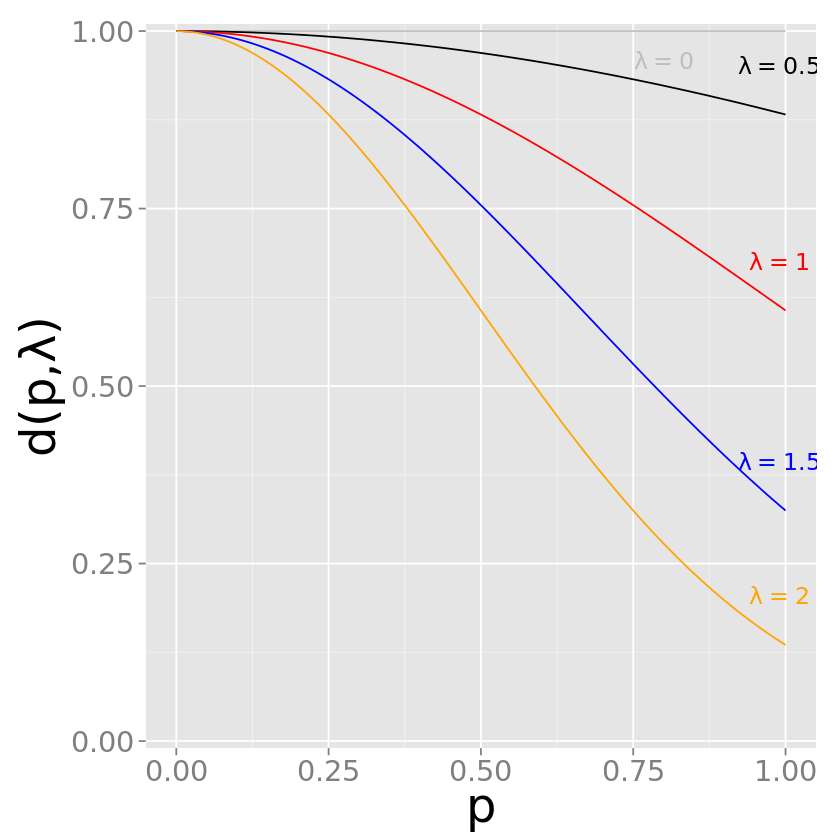
\includegraphics[width=0.3\textwidth]{graphs/ch7/decay-gauss.png}
}
\subfloat[Exponential \label{subfig7:exp}]{%
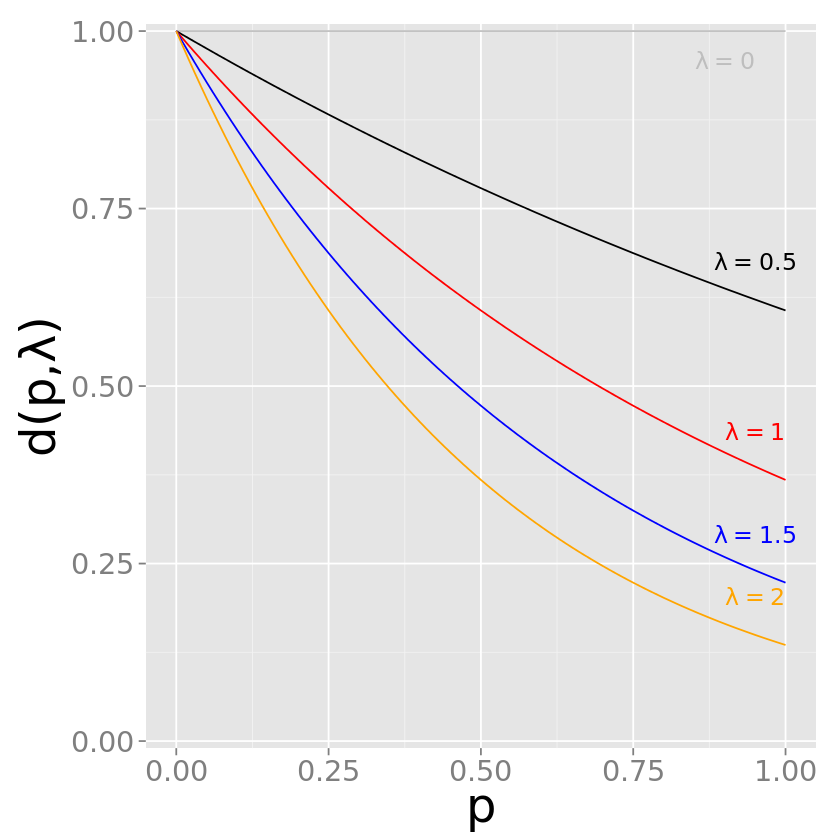
\includegraphics[width=0.3\textwidth]{graphs/ch7/decay-exp.png}
}
%\hfill
\subfloat[Windowed ($\delta_{win}$) \label{subfig7:windowed}]{%
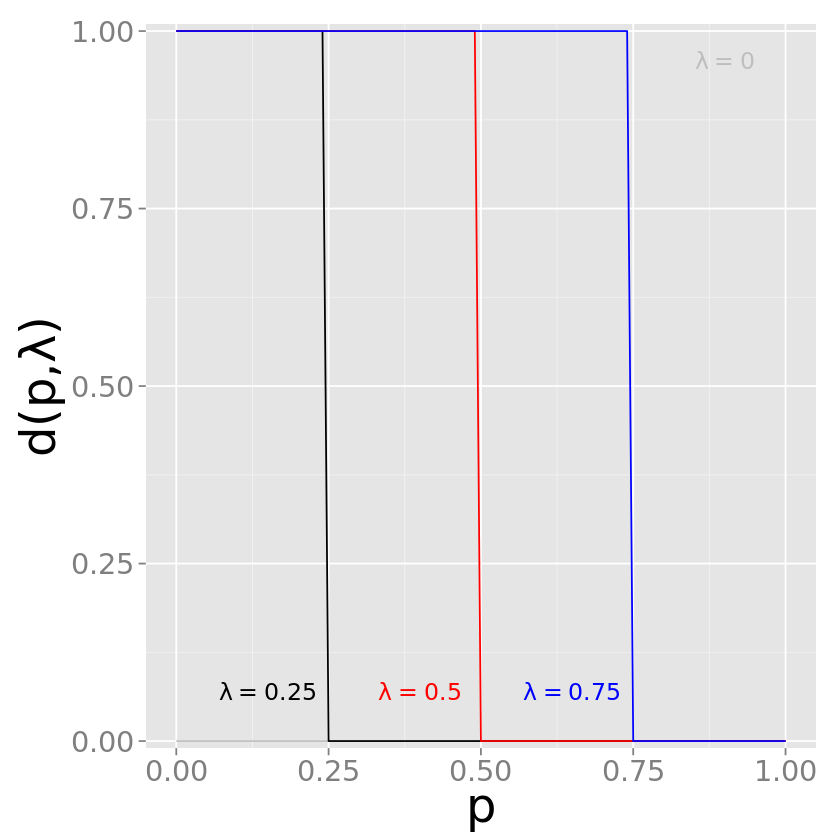
\includegraphics[width=0.3\textwidth]{graphs/ch7/decay-window.png}
}
\end{center}
\caption[Decay function examples]{Decay function examples \label{fig7:examples}}
\end{figure}

\subsection{Decaying Cache Frequencies}
As mentioned, the computation of the cache frequencies can incorporate a decay function $\delta(\cdot)$.  In keeping with the notion of locality of repetition, the closer a word occurs to the current utterance, the more it ought to effect the likelihood of the current word.   In Chapter~\ref{sec:classification}, application of decay functions to the computation of bags-of-words frequencies had a significant impact on classification tasks.  However, when applied to the cache component of the language model for the retrieval or transcription task, we find no significant difference in performance between the decay-weighted cache versus whole-document cache ($\delta_0$).   

 
\begin{table}
\centering
\begin{tabular}{lclllll} \toprule
   \textbf{Language} ($\mathcal{T})$ & \textbf{Baseline} & \textbf{Decay} & \multicolumn{4}{c}{\textbf{TWV}}  \\ %\midrule 
   & \textbf{TWV} & $\lambda_{win}$ & 1.0\footnotemark & 0.75 & 0.5 & 0.25 \\
   & & $\lambda_{gauss,exp}$ & 0.5 & 1.0 & 1.5 & 2.0 \\ \midrule
Tagalog (50) & 0.244 & $\delta_{win}$ & \textbf{0.257}  & 0.258 & 0.258 & \textbf{0.262} \\
  & & $\delta_{gauss}$ & 0.258 & 0.258 & 0.257 & 0.258 \\
  & & $\delta_{exp}$ & 0.257 & 0.257 & 0.258 & 0.258 \\  
Vietnamese (200) & 0.254 & $\delta_{win}$ & \textit{0.254} & 0.254 & 0.254 & 0.255  \\
& & $\delta_{gauss}$ & 0.2540 & 0.254 & 0.254 & 0.254 \\
&& $\delta_{exp}$ & 0.254 & 0.254 & 0.253 & 0.254 \\
Zulu (100) &  0.270 & $\delta_{win}$ & \textbf{0.281} & 0.281  & 0.281 & 0.280 \\
& & $\delta_{gauss}$ & 0.276 & 0.281 & 0.281 & 0.280 \\
& & $\delta_{exp}$ & 0.281 & 0.281 & 0.281 & 0.281 \\
Tamil (100) & 0.216 & $\delta_{win}$ & \textbf{0.229} & 0.228 & 0.228 & 0.226 \\
& & $\delta_{gauss}$ & 0.229 & 0.228 & 0.228 & 0.228 \\
& & $\delta_{exp}$ & 0.228 & 0.228 & 0.228 & 0.228 \\
        \bottomrule
\end{tabular}
\caption[TWV effects of decaying cache frequencies]{TWV effects of applying decaying cache frequencies to lattice re-scoring, compared with the baseline N-gram language model. \label{fig7:decay}}
\end{table}


\footnotetext{Corresponds to $\delta_0$}


\begin{table}
\centering
   \begin{tabular}{lcllllll} \toprule
   \textbf{Language} ($\mathcal{T})$ & \textbf{Baseline}  & \textbf{Decay} & \multicolumn{4}{c}{\textbf{WER (\%)}}  \\ %\midrule 
   & \textbf{WER} & $\lambda_{win}$ & 1.0 & 0.75 & 0.5 & 0.25 \\
   & & $\lambda_{gauss,exp}$ & 0.5 & 1.0 & 1.5 & 2.0 \\ \midrule
Tagalog (50) & 59.8 & $\delta_{win}$ & 59.8 & 59.8 & 59.7 & 59.7\\
  && $\delta_{gauss}$ & 59.8 & 59.8 & 59.7 & 59.7 \\
  && $\delta_{exp}$ & 59.8 & 59.7 & 59.8 & 59.8 \\
Vietnamese (200) & 62.0 & $\delta_{win}$ & 61.9 & 62.0 & 62.0 & 62.0  \\
&& $\delta_{gauss}$ & 62.0 & 61.9 & 61.9 & 62.0 \\
&& $\delta_{exp}$ & 61.9 & 62.0 & 62.0 & 62.0 \\
Zulu (100) & 67.6 & $\delta_{win}$ & 67.3 & 67,2 & 67.2  & 67.2 \\
&& $\delta_{gauss}$ & 67.2 & 67.2 & 67.2 & 67.2 \\
&& $\delta_{exp}$ & 67.3 & 67.2 & 67.2 & 67.3 \\
Tamil (100) & 75.8 & $\delta_{win}$ & 75.5 &  75.5 &  75.5 & 75.5 \\
&& $\delta_{gauss}$ & 75.5 & 75.5 & 75.5 & 75.5 \\
&& $\delta_{exp}$ & 75.5 & 75.5 & 75.5 & 75.4 \\ \bottomrule
\end{tabular}
\caption[WER effects of decaying cache frequencies]{WER effects of applying decaying cache frequencies to lattice re-scoring, compared with the baseline N-gram language model \label{fig7:decayWER}}
\end{table}

Table~\ref{fig7:decay} shows retrieval performance for lattice re-scoring in terms of the NIST TWV metric for the different decay models over the baseline N-gram model.   Table~\ref{fig7:decayWER} shows the transcription performance in terms of WER.   We restrict  our analysis of the decay-weighted cache models to those models whose number of latent topics $\mathcal{T}$ performed best overall in terms of the retrieval task.  The $\lambda$ parameter for the windowed `decay' function $\delta_{win}$ is given in descending order as it is a threshold and not a decay rate, and so moving left to right the cache frequencies are effectively computed from a decreasing fraction of the current document (illustrated graphically in  Figure~\ref{fig7:examples}).  Given the limited impact of the various decay functions (in general < 0.1\% absolute in each metric), the rest of our experiments are reported with the full non-decaying cache frequencies.


\subsection{Re-scoring and Re-decoding}

When we compare performance between re-scoring and re-decoding using our cache-augmented models, we again observe the same positive effect that we saw in section~\ref{sec:ltlm} on retrieval accuracy (TWV and lattice recall) and for Tamil and Zulu, recognition accuracy (WER).  Table~\ref{fullRes} presents the accuracy results in terms of TWV, Table~\ref{fig7:lrecall} shows results for the same systems in terms of lattice recall (the overall percentage of keyword occurrences captured in the ASR lattices), and Table~\ref{fig7:WER} shows the results in terms of WER.  

If we look specifically at lattice recall (Table~
\ref{fig7:lrecall}), we observe 2.5 to 5 \% absolute increase in recall in the unigram case (depending on the language), and from 0.7\% to 4.6\% in the bigram cache case.  These results are consistent with the results in Chapter 4 with the topic-only (LDA) augmented models, and supports the premise that by boosting keywords with lower probability under the baseline N-gram  model, they survive the decoder pruning low-likelihood paths from the lattice.    


%The and also to consider the effect of a bigram versus unigram cache.



\begin{table}
\centering
   \begin{tabular}{lrrrr} \toprule
   \textbf{Language} & $\mathcal{T}$ & \textbf{Baseline} & \multicolumn{2}{c}{\textbf{Lattice Recall (\%) }} \\
   & & & \textbf{1-gram} & \textbf{2-gram} \\ \midrule
	Tagalog & 50 & 77.8 & 79.8 & 79.0 \\ 
	   \rowcolor{blue!5}	& 100 & &\textbf{79.8} & 79.3 \\
		& 150 & & 79.3 & 79.0 \\
		& 200 & & 79.3 & 79.0\\
	   \rowcolor{blue!5} Vietnamese & 50 & 55.4  & \textbf{57.1} & 56.6 \\
	         & 100 & & 56.3 & 56.5 \\
	         & 150 & & 56.5 & 56.4 \\
	         & 200 & & 56.7 & 56.1\\
	Zulu   & 50&  71.7 & 74.2 & 73.1 \\
   \rowcolor{blue!5}	& 100 & & \textbf{74.3} & 73.3 \\
	& 150 & & 74.1 & 73.1\\
	& 200 & & 74.2 & 73.1\\
	Tamil &  50 & 57.3 & 62.3 & 61.5 \\ 
   \rowcolor{blue!5} & 100 & &\textbf{ 62.3} & 61.9 \\
	& 150 & & 62.6 & 61.7 \\
	& 200 &  & 62.4 & 61.8 \\\bottomrule
	
    \end{tabular}
\caption[Improvements in Lattice Recall with joint cache-topic models]{Improvements in Lattice Recall when decoding with cache-augmented topic language models. \label{fig7:lrecall}}
\end{table}

We have highlighted the rows for which choice of $\mathcal{T}$ resulted in the highest lattice recall per language (Tagalog:100, Vietnamese:50, Zulu:100, and Tamil:100).   However for Tagalog and Vietnamese those choices for $\mathcal{T}$ did not result in the highest overall retrieval accuracy (again, highlighted similarly in Table~\ref{fullRes}).  

The bigram cache model (used for re-decoding) consistently underperformed the unigram cache model in terms of lattice recall and in terms of TWV.  The difference is not as evident for lattice re-scoring, but it is clear that the bigram cache is not offering any additional benefit.

\begin{table}
\centering
   \begin{tabular}{lrrrrr} \toprule
   \textbf{Language} & $\mathcal{T}$ &  \multicolumn{2}{c}{\textbf{Re-score}} & \multicolumn{2}{c}{\textbf{Re-decode}}\\ 
   & & 1-gram  & 2-gram & 1-gram  &  2-gram \\ \midrule 
   Tagalog & \multicolumn{5}{l}{ N-grams: 0.244 \hfill Trigger: 0.161 } \\ 
   \rowcolor{blue!5}	  & 50 & 0.257 & 0.257 & \textbf{0.261}  & 0.258 \\ 
		& 100 & 0.256 & 0.258 & 0.258 & \textbf{0.260} \\
		& 150 & 0.254 & 0.255 & 0.257 & 0.256 \\
		& 200 & 0.257 & 0.253 & 0.254 & 0.258 \\ \midrule
   Vietnamese & \multicolumn{5}{l}{ N-grams: 0.254 \hfill Trigger: 0.190 } \\
	 & 50 & 0.256 & \textit{0.253} & 0.267 & 0.260 \\
	 & 100 & 0.254 & 0.253 & 0.265 & 0.259 \\
	 & 150 & 0.255 & 0.256 & 0.264 & 0.261 \\
   \rowcolor{blue!5} & 200 & 0.254 & 0.254 & \textbf{0.269} & 0.263\\ \midrule
   Zulu & \multicolumn{5}{l}{ N-grams: 0.270 \hfill Trigger: 0.192 } \\
    & 50 & 0.272 & 0.272 & 0.285  & 0.275\\
   \rowcolor{blue!5} & 100 & 0.281 & 0.277 & \textbf{0.287} & 0.280 \\
	& 150 & 0.277 & 0.279 & 0.282  & 0.278 \\
	& 200 & 0.279  & 0.279 & 0.284 & 0.278 \\ \midrule
   Tamil & \multicolumn{5}{l}{ N-grams: 0.216 \hfill Trigger: 0.138 } \\	
	&  50 & 0.225 & 0.225 & 0.240  & 0.234 \\ 
   \rowcolor{blue!5} & 100 & 0.229 & 0.226 & \textbf{0.241} & 0.238 \\
	& 150 & 0.228 & 0.223 & 0.237 & 0.236 \\
	& 200 & 0.228 & 0.225 & 0.240 & 0.237 \\\bottomrule
	
    \end{tabular}
\caption[Effect of cache-augmented topic model on TWV]{Effect on Term Weighted Value (TWV) of applying cache-augmented topic model\label{fullRes}}
\end{table}

\begin{table}
\centering
%   \begin{tabular}{lrrrrr} \toprule
%   \textbf{Language} & $\mathcal{T}$ &  %\multicolumn{2}{c}{$\mathbf{\kappa}$\textbf{LDA Unigram}} & \multicolumn{2}{c}{$\mathbf{\kappa}$\textbf{LDA Bigram}}\\ 
%   & & Re-score & Decode & Re-score &  Decode \\ \midrule 
%   Tagalog & \multicolumn{5}{l}{ N-grams: 60.0 \hfill Trigger: 61.7 } \\ 
%	 & 50 & 59.8 & 59.8 & \textbf{59.6} & 59.7 \\ 
%	  & 100 & 60.0 & 60.0 & 59.8 & 59.8 \\
%	  & 150 & \textit{60.2} & \textit{60.1} & 59.9 & 60.0\\
%	  & 200 & \textit{60.3} & \textit{60.3} & 60.0 & 60.1\\ \midrule 
%	Vietnamese & \multicolumn{5}{l}{ N-grams: 62.0 \hfill Trigger: 63.7 } \\ 
%	  & 50 & 61.9 & 61.9 & 61.8 & 61.8 \\
%	  & 100 & 61.9 & 61.9 & 61.8 & 61.9 \\
%	  & 150 & 61.9 & 61.9 & 61.8 & 61.9 \\
%	  & 200 & 61.9 & 62.0 & 61.8 & 61.9\\ \midrule 
%	Zulu & \multicolumn{5}{l}{ N-grams: 67.6 \hfill Trigger: 69.2 } \\ 
 %  \rowcolor{blue!5} & 50& 67.2 & \textbf{67.1} & 67.2 & 67.1 \\
%	& 100 & 67.3 & 67.2 & 67.2 &  67.2 \\
	%& 150 & 67.5 & 67.2 & 67.3 & 67.2 \\
%	& 200 & 67.2 & 67.2 & 67.4 & 67.3 \\ \midrule 
%	Tamil & \multicolumn{5}{l}{ N-grams: 75.8 \hfill Trigger: 76.9 } \\
%	 & 50 & 75.5 & 75.5 & 75.4 & 75.4 \\ 
%   \rowcolor{blue!5} & 100 & 75.5 & \textbf{75.4} & 75.5 & 75.5 \\
%	& 150 & 75.5 & 75.5 & 75.4 & 75.4 \\
%	& 200 & 75.6 & 75.6 & 75.6 & 75,6 \\\bottomrule
%    \end{tabular}
   \begin{tabular}{lrrrrr} \toprule
   \textbf{Language} & $\mathcal{T}$ &  \multicolumn{2}{c}{\textbf{Re-score}} & \multicolumn{2}{c}{\textbf{Re-decode}}\\ 
   & & 1-gram & 2-gram & 1-gram &  2-gram \\ \midrule 
   Tagalog & \multicolumn{5}{l}{ N-grams: 60.0 \hfill Trigger: 61.7 } \\ 
	 & 50 & 59.8 & \textbf{59.6} & 59.8 & 59.7 \\ 
	  & 100 & 60.0  & 59.8 & 60.0& 59.8 \\
	  & 150 & \textit{60.2} & 59.9 & \textit{60.1} & 60.0\\
	  & 200 & \textit{60.3} & 60.0 & \textit{60.3}  & 60.1\\ \midrule 
	Vietnamese & \multicolumn{5}{l}{ N-grams: 62.0 \hfill Trigger: 63.7 } \\ 
	  & 50 & 61.9 & 61.8 & 61.9 & 61.8 \\
	  & 100 & 61.9 & 61.8 & 61.9  & 61.9 \\
	  & 150 & 61.9 & 61.8 & 61.9 & 61.9 \\
	  & 200 & 61.9 & 61.8 & 62.0 & 61.9\\ \midrule 
	Zulu & \multicolumn{5}{l}{ N-grams: 67.6 \hfill Trigger: 69.2 } \\ 
   \rowcolor{blue!5} & 50& 67.2 & 67.2 & \textbf{67.1} & 67.1 \\
	& 100 & 67.3 & 67.2 & 67.2 &  67.2 \\
	& 150 & 67.5 & 67.3 & 67.2 & 67.2 \\
	& 200 & 67.2 & 67.4 & 67.2 & 67.3 \\ \midrule 
	Tamil & \multicolumn{5}{l}{ N-grams: 75.8 \hfill Trigger: 76.9 } \\
	 & 50 & 75.5 & 75.4 & 75.5 & 75.4 \\ 
   \rowcolor{blue!5} & 100 & 75.5 & 75.5 & \textbf{75.4} & 75.5 \\
	& 150 & 75.5 & 75.4 & 75.5 & 75.4 \\
	& 200 & 75.6 & 75.6 & 75.6 & 75.6 \\\bottomrule
	
    \end{tabular}    
\caption[Effect of cache-augmented topic model on WER]{Effect on Word Error Rate (\%) of applying cache-augmented topic model \label{fig7:WER}}
\end{table}

Retrieval in all languages is improved by decoding with the cache-augmented topic model.  With respect to recognition, the results varied widely depending on language.   The WER of the Tamil and Zulu systems were improved by the ungram models by 0.5\% and 0.4\% absolute over the baseline, whereas Vietnamese improved by at most 0.2\% and Tagalog was actually worsened by up to 0.3\% absolute.   % consistent with chapter 3?
% fusion experiment?  2 topic models

Given these full sets of results we conclude by comparing the best results of Table~\ref{fullRes} with the LDA results from Chapter 4 on a language by language basis (cf. Figure~\ref{fig7:ldaklda}).  We can visualize the impact of adding the local context from the cache probabilities in addition to the latent topic models by comparing the LDA versus $\kappa$LDA figures.  As with our previous work in Chapter 4 we see incremental improvements with the cache information in addition the latent topics in all languages except for Vietnamese.  Similarly in Tagalog, we see, as before, the cache information has a proportionally larger effect relative to the latent topics.  Nonetheless, we maintain the same conclusion, given the evidence across all four languages, that the topic and cache contexts provide complementary information, effective in boosting keyword retrieval.

\begin{figure}
\centering
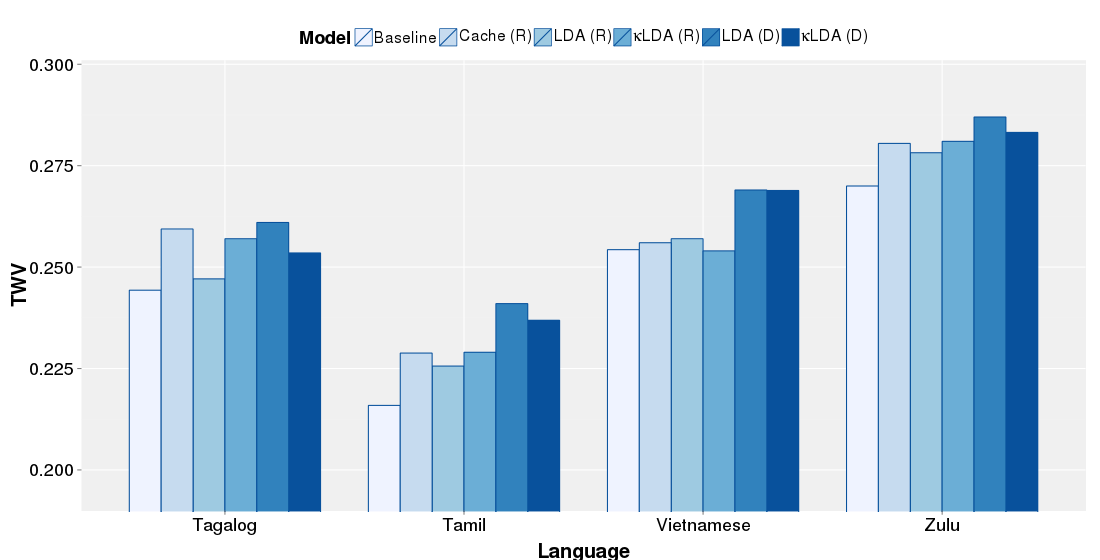
\includegraphics[width=\textwidth]{graphs/ch7/compare.png}
\caption[Comparison of $\kappa$LDA with LDA]{Comparison of $\kappa$LDA retrieval performance with LDA \label{fig7:ldaklda}}
\end{figure}

\section{Conclusions}

In conclusion, we have demonstrated that our joint cache-augmented topic model captures similar improvements in keyword retrieval to the ad hoc approach described in Chapter 4.  By modeling both broad and local contexts in a single model, we arrived at the same result with one fewer passes over the data.  

We found no additional benefit from a bigram cache.  However, as we have focused primarily on the limited resource setting, we intend to extend this work to larger training corpora.  As we suggested, bigram cache estimates for more accurate ASR output may in fact be beneficial,  however this may be offset by a more accurate N-gram language model overall.

We address our initial constraints of large data volumes and language diversity with a model that improves accuracy in the low resource setting, and we improve computational efficiency without sacrificing retrieval accuracy by moving from a two pass model to a single joint model.
